% 2013 湖南卷理科第 18 题：直角边长 4 米的三角形地块及格点作物（TikZ 矢量重绘）。
% 格点为满足 x,y>=0, x+y<=4 的整点，共 15 个。
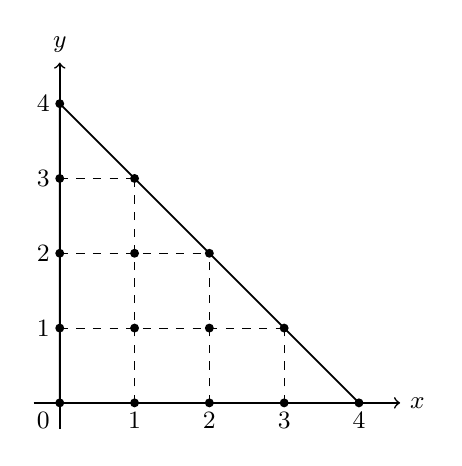
\begin{tikzpicture}[scale=0.95, font=\small, line width=0.6pt]
  \draw[->] (-0.35,0) -- (4.55,0) node[right] {$x$};
  \draw[->] (0,-0.35) -- (0,4.55) node[above] {$y$};
  \node[below left] at (0,0) {$0$};

  \begin{scope}
    \clip (0,0) -- (4,0) -- (0,4) -- cycle;
    \foreach \i in {1,2,3} {
      \draw[dashed, line width=0.35pt] (\i,0) -- (\i,4);
      \draw[dashed, line width=0.35pt] (0,\i) -- (4,\i);
    }
  \end{scope}

  \draw (0,0) -- (4,0) -- (0,4) -- cycle;

  \foreach \x in {1,2,3,4} {
    \node[below] at (\x,0) {$\x$};
    \node[left] at (0,\x) {$\x$};
  }
  \foreach \x in {0,...,4} {
    \foreach \y in {0,...,4} {
      \ifnum\numexpr\x+\y\relax<5
        \fill (\x,\y) circle (1.7pt);
      \fi
    }
  }
\end{tikzpicture}
